\chapter{GNL モデルにおける集計ルールの導出}
\def\thesection{\thechapter.\arabic{section}}
\setcounter{section}{0} 
\section{7 章の目的}
離散選択モデルの構築において,どの単位で離散的な選択肢とすべきかという点は重要である.
例えば,コカ・コーラというブランドを一つの選択肢にすべきか,ペットボトルのコーラという商品容器の違いを一つの選択肢とすべきかということである.
これらはそれぞれの選択肢集合においてモデルを構築することが可能であるが,一般的な効用関数形,特に線形の場合においても,ある選択肢同士を一つの選択肢として束ねると,束ねる前後で選択確率の整合性が取れなくなってしまう.
このような問題は通称集計問題と呼ばれ,特に立地選択や目的地選択において問題とされている.
これらの選択問題において問題とされる理由として,空間上の広がりは実質的には連続で,離散ではないことが挙げられる.
つまり,データの入手可能性を無視すれば,町丁目,メッシュ等いかようにもゾーンを設定できてしまう.

選択肢が本質的に連続的ではなく離散的なブランド選択モデルにおいても,どのレベルで選択肢集合を構築するべきか,
またその場合,異なる選択肢集合間で整合性が取れるのかという問題が存在する.
特に,選択肢が多数存在する場合には,分析対象以外の商品については束ねることにより,なるべく選択肢を少なくしたい.
これは,分析者が分析に要する時間,労力を減らすという点以外にも,実際の消費者が並行して多くの選択肢を比較,検討できないという心理学的特性 (Miller, 1956 \cite{Mil56}) をも反映しているものとなる.

本章では,前章までに引き続き Generalized Nested Logit (GNL) モデルにおいて,集計問題を回避するための集計ルールを提示する.
これにより,GNL モデルにおいて容易に選択肢の併呑することにより選択肢の減少が可能になり,ひいては分析が容易になる.
一般的に GNL モデルは選択肢数の増加によるパラメータ数の増加が著しいため,集計の効果は大きい.
集計ルールの導出により無駄な計算が省かれ,パラメータ推定の計算時間,負荷の削減に寄与することとなる.

本章では,マーケティング・サイエンスにおいて多く用いられている一般的なブランド選択モデルを例に,集計問題を回避する集計ルールを導出する.
ここで集計的とは,単に集計的ではなく,理想的消費者の選択行動をミクロ経済学の効用理論に基づいて記述し,この理想的消費者である個人,あるいは全体の行動を指す.
また,その拡張として,先行研究で行なわれている目的地と交通機関を選択する交通機関選択モデルにおける GNL モデルの集計ルールを導出する.

本章の先行研究として,Sweet (1997) \cite{Swe97},Ivanova (2005) \cite{Iva05} が挙げられる.
Sweet,Ivanova はそれぞれ GNL モデルの基となる MNL, NL モデルについて集計問題を克服できる集計ルールを示している.
ただしSweet,Ivanova は,最初に目的地を選択し,次に交通機関を選択するというステップを踏む限定的な交通機関選択モデルにおけるネストの集計ルールを示しており,
構造面では一例を示しているに過ぎない.
GNL モデルは 既に示した MNL, NL, CNL, PCL の各モデルだけではなく,商圏分析や商業施設計画で広く用いられている Huff モデル\cite{Huf64} についても同様の条件を示していることとなる.
これは Huff モデルが MNL モデルに内包されるためである.

本章では,集計ルールの導出に Sweet の条件を利用する.
この条件は MNL モデルのもとでのルールであり,GNL モデルに適用するためには若干の修正が必要である.
Ivanova は,これを NL モデルに適用する際に拡張しているものの,明示的に示してはいない.
この条件についても本章で検討する.

本章の構成は次のとおりである.
まず,第 2 節において GNL モデルにおいて集計問題が発生し,単純な集計ルールが適用できないことをブランド選択モデルを例に示す.
次に第 3 節で,集計ルールが満たすべき条件について示す.
第 4 節は本章の核心であり,実際に GNL モデルにおいて集計問題を克服可能な集計ルールを,
ブランド選択モデルとして 1) ネストを集計化したもの,2) 選択肢を集計化したもの,3) 交通機関選択モデルとしてネストを集計化したもの
の計三つの場合において求める.
第 5 節は,4 節で得られた GNL モデルにおける集計ルールと,MNL,NL の各モデルにおけるルールとの比較,考察である.
そして最後に第 6 節で結論と今後の課題について述べる.
%****************************************************************************************************************************************
\section{GNL モデルにおける集計問題の生起例}
本節では,実際に GNL モデルにおいて集計問題が発生し,直感的に思いつく集計ルールでは克服できないことを例(ブランド選択モデル:ペットボトル・コーラ)を用いて説明しよう.
ここで用いるデータ,設定は 4 章,5 章もしくは Takahashi (2011) \cite{Tak11} ,高橋 (2012) \cite{Tak12} で用いたものである.

選択肢数は八つ,そしてその選択構造は図 \ref{fig:7-1} 左図に示すように,ネスト数六つの構造としよう.
ここでのネスティング・ルールはブランド(商品)が持つ属性(値)をネストとする属性分割を用いている.
ブランド $k$ の確定的効用は,次に示す線形の効用関数とする:
\begin{equation}
V_k^h=\alpha_1 X_{1k} + \alpha_2 X_{2k} + \alpha_3 X_{3k} + \alpha_4 X_{4k} + \alpha_5 X_{5k}.
\end{equation}
ここで, $X_{1k}$ は $k$ の価格,  $X_{2k}$ はブランド・ダミー (Coca-Cola $= 1$, Pepsi $= 0$),$X_{3k}$ は $k$ の容量, $X_{4k}$ は低糖・無糖ダミー(低糖・無糖$ = 1$, 普通$ = 0$),
$X_{5k}$ は前回購買ダミー (前回購買商品 $= 1$, それ以外 $= 0$),$\alpha_i$ は $i$番目の変数に対応するパラメータである.  
また,類似度パラメータは煩雑な議論を避けるため,$\mu_j = \mu_J := \mu~~\forall j,J$ とする.
スキャン・パネル・データより最尤推定した集計前のパラメータは 表 \ref{tb:7-1} に示すとおりである.

\begin{figure*}[!t]
 \begin{center}
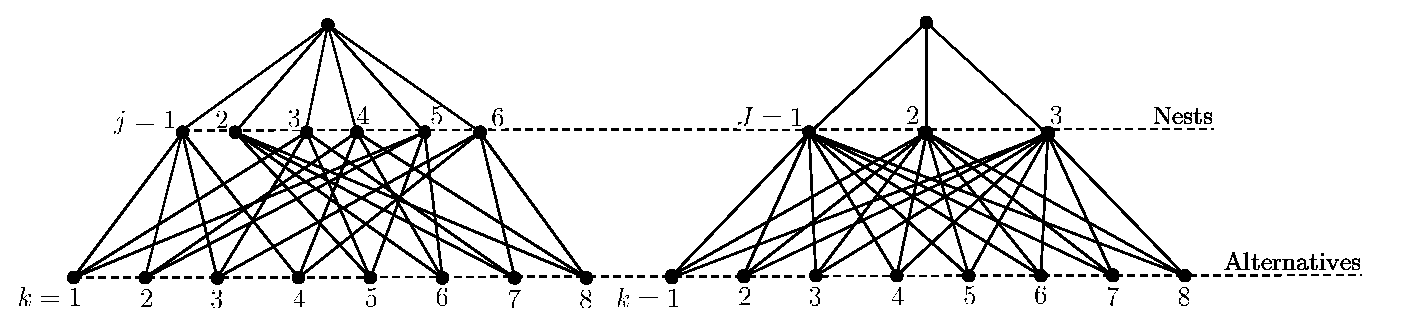
\includegraphics[width=160mm]{clip7-1.eps}
 \caption{集計問題生起例における GNL モデルの構造}
 \label{fig:7-1}
 \end{center}
\end{figure*}

\begin{table}
\begin{center}
\caption{選択構造例において最尤推定されたパラメータ} \label{tb:7-1}
\begin{tabular}{crcrcrcrcr}
\toprule\noalign{\smallskip}
Para.&Value&Para.&Value&Para.&Value&Para.&Value&Para.&Value
\\\noalign{\smallskip} \hline\hline
$\alpha_1$ & $-0.0147$ & $\gamma_{11}$ & $0.4760$ & $\gamma_{31}$ & $0.1038$ & $\gamma_{52}$ & $0.0061$ & $\gamma_{72}$ & $0.1604$\\
$\alpha_2$ &  $0.4755$ & $\gamma_{13}$ & $0.1149$ & $\gamma_{33}$ & $0.4621$ & $\gamma_{53}$ & $0.6821$ & $\gamma_{73}$ & $0.8396$\\
$\alpha_3$ &  $0.0021$ & $\gamma_{15}$ & $0.4091$ & $\gamma_{36}$ & $0.4341$ & $\gamma_{55}$ & $0.3118$ & $\gamma_{76}$ & $0.0000$\\
$\alpha_4$ & $-0.3597$ & $\gamma_{21}$ & $0.7870$ & $\gamma_{41}$ & $0.2955$ & $\gamma_{62}$ & $1.0000$ & $\gamma_{82}$ & $0.0357$\\
$\alpha_5$ & $0.8506$ & $\gamma_{24}$ & $0.1001$ & $\gamma_{44}$ & $0.0346$ & $\gamma_{64}$ & $0.0000$ & $\gamma_{84}$ & $0.1129$\\
$\mu$      & $0.4650$ & $\gamma_{25}$ & $0.1129$ & $\gamma_{46}$ & $0.6700$ & $\gamma_{65}$ & $0.0000$ & $\gamma_{86}$ & $0.8514$\\
\bottomrule
\end{tabular}
\end{center}
\end{table}

実際に集計化する上で,ネスト $1,2;3,4;5,6$ を集計化することを具体的に考えよう.
すなわち,図 \ref{fig:7-1} 右図の構造に集計化するものとする.
ここでは,
\vspace{3.0mm}
\begin{description}
\item [\mbox{}{\bf ルール 1 算術平均}] \mbox{}$ \check V_J^h = \frac{\sum_{j \in J} \check  V_j^h}{N_J}$,
\item [{\mbox{}\bf ルール 2 幾何平均}] \mbox{}$ \check V_J^h = \left(\prod_{j \in J} \check  V_j^h \right)^{1/N_J}$
\end{description}
\vspace{3.0mm}
の適用を試みる.ルール 1 は誰しもが一番最初に思いつくであろうもの,ルール 2 は効用項が $\exp$ の肩の上に乗っていることを反映したものである.
ここで,$\check V_j$ は,
\begin{align}
\check V_j^h := \sum \limits_{k^{\prime} \in {\cal K}_j} \left( \gamma_{k^{\prime}j}\exp \left({ V_{jk^\prime}^h + \hat V_{k^\prime}^h } \right) \right)^{1/\mu_j}
\end{align} 
である.$\check V_j^h$ と $\tilde V_{j}^h$,$V_j^{\prime h}$ の関係は,式\eqref{eq2-52} を参照せよ.また,$N_J$ は集計後のネスト $J$ に属する集計前のネスト $j$ の数である.

\begin{table}[t]
\begin{center}
\caption{間違った集計ルールの適用例} \label{tb:7-2}
\begin{tabular}{cccc}
\toprule
$j$ & $P_j^{\A}$ & $P_J^{\A}$(Rule 1) & $P_J^{\A}$(Rule 2)\\
\hline\hline
$1$& $0.239$ & \multirow{2}{3cm}{$0.324(5.2\%)^{\ast}$} & \multirow{2}{3cm}{$0.392(14.6\%)$} \\
$2$& $0.103$ &&\\
$3$& $0.303$ &\multirow{2}{3cm}{$0.376(16.8\%)$} & \multirow{2}{3cm}{$0.190(41.1\%)$} \\
$4$& $0.018$ &&\\
$5$& $0.196$ &\multirow{2}{3cm}{$0.300(10.8\%)$} & \multirow{2}{3cm}{$0.419(24.5\%)$} \\
$6$& $0.140$ &                                               &                                                \\
\hline
$k$ & $Q_k^{\A}$ & $Q_K^{\A}$(Rule 1) & $Q_K^{\A}$(Rule 2)\\
\hline \hline
$1$& $0.303$ & $0.326(7.9\%)$ & $0.404(33.5\%)$\\
$2$& $0.095$ & $0.091(4.8\%)$ & $0.109(14.6\%)$\\
$3$& $0.139$ & $0.131(6.0\%)$ & $0.129(8.3\%)$\\
$4$& $0.037$ & $0.028(25.4\%)$ & $0.038(2.4\%)$\\
$5$& $0.208$ & $0.242(16.5\%)$ & $0.174(16.4\%)$\\
$6$& $0.092$ & $0.049(53.0\%)$ & $0.063(31.9\%)$\\
$7$& $0.103$ & $0.119(15.3\%)$ & $0.064(38.2\%)$\\
$8$& $0.023$ & $0.014(37.6\%)$ & $0.020(13.9\%)$\\
\bottomrule
\multicolumn{4}{l}{$\ast$()内は集計前との相対誤差を表わす.}
\end{tabular}
\end{center}
\end{table}

それぞれ集計前,集計後の各選択肢,ネストの選択確率は表 \ref{tb:7-2}のとおりである.
ネスト $j$,商品 $k$ どちらのレベルにおいても,単純な算術平均や幾何平均による集計ルールは
選択割合(確率)の整合性がとれていないことがわかる.
特に,選択確率が小さい選択肢 $6$ の選択割合 $Q_6^{\A}$ は集計ルールの非整合性による影響が大きく,相対誤差がルール 1 では $53.0\%$,ルール 2 でも$31.9\%$ と大きくなっている.
つまり,整合的な集計ルールとは,算術,幾何平均のような単純なルールではない.

%****************************************************************************************************************************************
\section{集計ルールが満たすべき条件}
Sweet は集計が整合的に行われているために満たすべき条件として,MNL モデルのもとで,次の二つの条件を示している.
\begin{description}
\item [{\bf 条件 $1$ 固定需要}]  個人 $h$ が集計化された選択肢 $K$ を選ぶ周辺確率 $Q_K^h$ は,集計化前の選択肢 $k$ ($k$ は $K$ に包含されるものとする:$k \in K$)の効用 $V_k^h$ を
共通の効用である$V_{K}^{h}$に置き換えても変化がない.
\item  [\bf 条件 $2$ 選択確率の整合性] 個人 $h$ が集計化された選択肢 $K$ を選ぶ周辺確率 $Q_K^h$ は,集計化される前の選択肢 $k$ ($k \in K$) の選択確率と等しい:
\begin{equation}
Q_K^h = \sum \limits_{k \in K} Q_k^h.\label{eq7-1}
\end{equation}
\end{description}
これらの条件は,選択行動が $1$ 段階である MNL モデルの下での条件であることに留意されたい.
つまり,これをそのまま $2$ 段階の選択行動である NL,GNL の各モデルには適用できない.

Ivanova はこれらの条件を拡張し,NL モデルに適用している.
Ivanova では,ネスト $j$ について集計化しているモデルについて考えているが,
条件 $2$ をネスト $j$ 及び選択肢 $k$ について計 $2$ 回適用をしている.

本研究で対象とする GNL モデルでは,これ以外に,アロケーション・パラメータの条件が必要となる.
ここでは,次の条件を提示する:
\begin{description}
\item [{\bf 条件 $3$ アロケーション・パラメータの整合性}]
ネスト $j$ が $J$ に集計化された場合($j \in J$),アロケーション・ パラメータは次の条件を満たす必要がある:
\begin{equation}
\gamma_{kJ} = \sum_{j \in J} \gamma_{kj},\forall k. \label{eq7-2}
\end{equation}
\end{description}
条件 3 は集計が式\eqref{eq7-7}と整合的であるための条件である.
ただし,これはネストが集計化される場合についてのみの条件であり,選択肢が集計化される場合には適用することができない.

%****************************************************************************************************************************************
\section{GNL モデルにおける集計ルールの導出}
本節では,まず $1$ 回の集計を行なうブランド選択モデルにおいて,1) ネストの集計,2) 選択肢の集計,それぞれの場合について集計ルールを示し,
1) の拡張として,出発地,目的地計 $2$ 回の集計を行なう,3) 交通機関選択モデルにおけるネストの集計について集計ルールを示す.
なお,ここから先は,すべて消費者を表わす上添字 $h$ が付くため,これを省略する.

\subsection{ブランド選択モデル 1 :ネストの集計}
ここでは集計例と同様に,まずネストとして商品構成要素 $j$ を選択し,次に商品 $k$ を選択するものとする.
ネスト(商品構成要素)を $j \in J$という表現を用いよう.ここで $j$ は統合前のネスト,$J$ は統合後のネストを意味している.

ここで求めるべき集計ルールとは,$\hat V_J$,$\hat V_J^{\prime}$,$\hat V_{Jk}$ に関しての条件を指す.
条件 2 をネスト $j$ に適用し, GNL モデルの選択確率式\eqref{eq2-46}に代入することにより,
\begin{align}
\exp \left( \tilde V_J + V_J^{\prime} \right) =\sum \limits_{j \in J} \exp \left( \tilde V_j + V_j^{\prime} \right) \label{eq7-3}
\end{align}
を得る.ここで,条件 $1$ より
\begin{align}
V_J^{\prime} = \ln \sum_{j \in J} \exp V_j^{\prime}~~~~\forall j
\end{align}
であるため,式\eqref{eq7-3}は,
\begin{align}
\exp \left( \tilde V_J + V_J^{\prime} \right) =\sum \limits_{j \in J} \exp \left( \tilde V_j + V_J^{\prime} \right) \label{eq7-4}
\end{align}
と書き直せる.ここで,式\eqref{eq7-4}より $\tilde V_J$ に関する部分を消去し,
\begin{align}
\tilde V_J= \ln \sum_{j \in J} \exp \tilde V_j  \label{eq7-5}
\end{align}
を得る.式\eqref{eq7-5} を式\eqref{eq7-4} に代入し,これを整理することにより,
\begin{align}
V_J^{\prime}= \ln \sum_{j \in J} \exp \left(\tilde V_j + V_{j}^{\prime}\right) - \ln \sum_{j \in J} \exp \tilde V_j \label{eq7-6}
\end{align}
を得る.さらに条件 2 を結合確率 $\hat Q_k(j)$,$\hat Q_k(J)$ について適用する:
\begin{align}
\sum_{ j \in J} \hat Q_k(j) = \hat Q_k(J). \label{eq7-7}
\end{align}
ここで,結合確率 $\hat Q_k(j)$,$\hat Q_k(J)$ は,
\begin{align}
\hat Q_k(j):=& P_j P_{k|j}, \label{eq7-8}\\
\hat Q_k(J) :=& P_J P_{k|J} \label{eq7-9}
\end{align}
なる確率である.読者は,Ivanova の NL モデルへの適用例を見て,
\begin{align}
\hat Q_k(j):=& \sum_{J=1}^{N_J} \sum_{j \in J} P_j P_{k|j} ,\\
\hat Q_k(J):=& \sum_{J=1}^{N_J} P_J P_{k|J}
\end{align}
として条件 $2$ が適用されるのではないかと考えるかもしれない.
しかし,このような適用の場合,$V_{Jk}$ に関する条件を明示的には求めることができなくなる.

ここで条件 $2$ が適用されるのは,本質的には $P_{k|j}$,$P_{k|J}$ に関してであり,$j \rightarrow k$ という「選択経路」ごとに集計ルールが適用されるべきである.
データとして $j$ が観測可能か否かに限らず,集計ルールとして「選択経路」ごとの整合性が必要である.
集計前の選択肢において $\hat P_j$ は計算されており,これと整合的に $P_J$ も計算される.
つまり,$Q_k$ について整合的であるルールは,$P_{j}$,$\P_{J}$ と $P_{k|j}$,$P_{k|J}$ がマルコフ性を有するため,残りの $P_{k|j}$,$P_{k|J}$ に関して整合的である必要がある.
これはブランド選択モデルだけではなく,交通機関選択モデルの出発地側も同様である.

式\eqref{eq7-7}は
\begin{align}
P_J P_{k|J} = \sum_{j \in J} P_j P_{k|j} \Longleftrightarrow P_{k|J} = \frac{\sum_{j \in J} P_j P_{k|j}}{\sum_{j^{\prime} \in J} P_{j^{\prime}}}\label{eq7-10}
\end{align}
と修正される.
式\eqref{eq7-10} は
\begin{align}
P_{k|J} = & \frac{\left( \gamma_{kJ}\exp \left( { V_{Jk}} + \hat V_{k} \right) \right)^{1/\mu_J}}
{\sum \limits_{k^{\prime} \in N_J} \left( \gamma_{k^{\prime}J}\exp \left( {V_{Jk^\prime}} + \hat V_k \right) \right)^{1/\mu_J}} 
= \frac{\left( \gamma_{kJ} \exp \left( V_{Jk} + \hat V_{k} \right) \right)^{1/\mu_J}}{\left( \exp V_J^{\prime} \right)^{1/\mu_J}}\notag\\
= & \frac{\sum_{j \in J} P_j P_{k|j}}{ \sum_{j^{\prime} \in J} P_{j^{\prime}}} \label{eq7-11}
\end{align}
と等価である.式\eqref{eq7-11}について対数を取り,$1/\mu_J$ で除すことにより,
\begin{align}
V_{Jk} = V_J^{\prime} - \hat V_k + \mu_J \ln \left( \frac{\sum_{j \in J} P_j P_{k|j}}{ \gamma_{kJ}^{1/\mu_J} \sum_{j^{\prime} \in J} P_{j^{\prime}}} \right)  \label{eq7-12}
\end{align}
を得る.最後に条件 $3$ を式\eqref{eq7-12}に代入し,
\begin{align}
V_{Jk} =& V_J^{\prime} - \hat V_k + \Upsilon, \label{eq7-13}\\
\Upsilon :=& \mu_J \ln \left( \frac{\sum_{j \in J} P_j P_{k|j}}{ \left( \sum_{j \in J} \gamma_{kj} \right)^{1/\mu_J} \sum_{j^{\prime} \in J} P_{j^{\prime}}} \right)  \label{eq7-14}
\end{align}
となる.

これらの式のうち,式\eqref{eq7-5},\eqref{eq7-6},\eqref{eq7-13}が,GNL モデルにおけるネストを集計した場合の満たすべき集計ルールとなる.
ここで注意すべきは,$\gamma_{kJ}$ と異なり,$\mu_J$ に関するルールは導出されないという点である.
これは,ネストごとの類似度パラメータが同一($\mu_J = \mu_j := \mu~~\forall j,J$)でない限り,集計後に新たに最尤推定もしくはその他の方法,ルールでパラメータ設定をしなければならないことを意味している.
%%%%%%%%%%%%%%%%%%%%%%%%%%%%%%%%%%%%%%%%%%%%%%%%%%%%%%%%%%%%%%%%%%%%%%%%%%%%%%%%%%%%%%%%%%%%%%%%%%%%%%%%%%%%%%%%%%%%%%%%%%%%%%%%%%%%%%%%%%%%%%%%%%%%%%%%%%%%%%%%%%%%%%%%%%%%%%%%%%%%%%%
\subsection{ブランド選択モデル 2 :選択肢の集計}
次に,ネストを構成する商品構成要素を集計するのではなく,選択肢であるブランドを集計する場合を考える.
ネストの集計と同様に,選択肢(ブランド)を $k \in K$ という表現を用いよう.ここで $k$ は統合前の選択肢,$K$ は統合後の選択肢を意味している.

ネストを集計した場合は,$\tilde V_J$,$V_J^{\prime}$,$\hat V_{Jk}$ に関しての条件三つが必要であったが,今回は $\hat V_{jK}$,$\hat V_K$ に関しての二つとなる.
条件 2 を$\hat P_{k|j}$,$\hat P_{K|j}$に適用することにより,
\begin{align}
&\left( \gamma_{Kj}\exp \left( V_{jK} + \hat V_K \right) \right)^{1/\mu_j} = \sum \limits_{k \in K} \left( \gamma_{kj} \exp \left( { V_{jk} + \hat V_k } \right) \right)^{1/\mu_j}\label{eq7-15}
\end{align}
を得る.ここで,条件 1 より,
\begin{align}
&\left( \gamma_{Kj} \exp \left( V_{jK} + \hat V_K \right) \right)^{1/\mu_j} = \sum \limits_{k \in K} \left( \gamma_{kj} \exp \left( { V_{jK} + \hat V_k } \right) \right)^{1/\mu_j}\label{eq7-16}
\end{align}
となる.式\eqref{eq7-16} を $\hat V_{K}$ について解くと,
\begin{align}
\hat V_{K} = \mu_j \ln \frac{1}{\gamma_{Kj}} \left( \sum \limits_{k \in K} \left( \gamma_{kj} \exp \hat V_{k} \right)^{1/\mu_j} \right) \label{eq7-17}
\end{align}
を得る.ちなみに式\eqref{eq7-17} の条件は,$\hat P_j^{\prime}$ に条件 $1$ を適用しても同様に得られる.
次に,式\eqref{eq7-17} を式\eqref{eq7-15} に代入し,整理すると,次の条件を得る:
\begin{align}
V_{jK} &= \mu_j \ln \left( \frac{1}{\gamma_{Kj}} \sum \limits_{k \in K} \left( \gamma_{kj} \exp V_{jk} \right)^{1/\mu_j} \right) - \mu_j \ln \left( \frac{1}{\gamma_{Kj}} \sum \limits_{k \in K} \left( \gamma_{kj} \exp \hat V_{k} \right)^{1/\mu_j} \right).  \label{eq7-18}
\end{align}

これらの式のうち,式\eqref{eq7-17},\eqref{eq7-18} が,GNL モデルにおけるブランド選択モデルでネストを集計した場合の満たすべき集計ルールとなる.
選択肢を集計化した場合には,ネストを集計化した場合のようなアロケーション・パラメータに関するルールは存在しない.
そのため,集計化に伴なう新たなパラメータ推定を行なうことを避ける意味において,説明変数により構造化した構造化 GNL モデル\cite{PB99} のような形で,アロケーション・パラメータを集計前に推定することが望ましい.
%%%%%%%%%%%%%%%%%%%%%%%%%%%%%%%%%%%%%%%%%%%%%%%%%%%%%%%%%%%%%%%%%%%%%%%%%%%%%%%%%%%%%%%%%%%%%%%%%%%%%%%%%%%%%%%%%%%%%%%%%%%%%%%%%%%%%%%%%%%%%%%%%%%%%%%%%%%%%%%%%%%%%%%%%%%%%%%%%%%%%%%
\subsection{交通機関選択モデル}
ここでは,まずネストとして目的地のゾーン $d$ を選択し,次に交通機関 $k$ を選択するモデルを考える.
交通計画分野に精通していない方にとっては,この選択構造(順番)は奇異に映るかもしれないが,
四段階推計法 (例えば\cite{Dob98}) のステップに準拠したものである.
当然,各交通機関の効用にはその交通機関により行くことが出来る目的地の効用が説明変数として加わることとなる.

交通機関選択モデルの場合,集計化された選択人数は出発地のゾーン $o$ ,目的地のゾーン $d$ を用い,
\begin{align}
H_k^o=&H^o Q_k^o = H^o  \sum_{d^{\prime}=1}^{N_d} \left( \frac{ \exp \left(\tilde V_{d^{\prime}}^o + V_{d^{\prime}}^{\prime o} \right)}
{\sum \limits_{d^{\prime \prime}=1}^{N_d} \exp \left(\tilde V_{d^{\prime \prime}}^o + V_{d^{\prime \prime}}^{\prime o} \right) }  \frac{\left( \gamma_{kd^{\prime}} \exp \left( V_{d^{\prime}k}^o + \hat V_{k}^o \right) \right)^{1/\mu_{d^{\prime}}}}
{\sum \limits_{k^{\prime} \in N_{d^{\prime}}} \left( \gamma_{k^{\prime}d^{\prime}} \exp \left(V_{d^{\prime}k^{\prime}}^{o} + \hat V_{k^{\prime}}^o \right) \right)^{1/\mu_{d^{\prime}}}} \right) \label{eq7-19}
\end{align}
と修正される.ここで, $H_k^o$ はゾーン $o$ において交通機関 $k$ を利用する人数,$H^o$ はゾーン $o$ を出発地とする人数,$Q_k^o$ はゾーン $o$ における交通機関 $k$ の選択確率であり,
式\eqref{eq7-1}--\eqref{eq7-7}と対応する部分についても上添字 $o$ がつく.
式\eqref{eq7-19}の意味するところは,交通機関選択モデルにおいては,選択確率における選択肢だけではなく,ゾーンの人数 $H^o$ についても集計化されるということである.
つまり,ブランド選択モデルで示した集計ルールはそのまま適用することができない.

前節までと同様に,ゾーンの集計化を $o \in O$,$d \in D$という表現を用いよう.ここで $o, d$ はネストを統合前,$O, D$ はネスト統合後のゾーンであり,
それぞれ $o, d$ は $O, D$ に統合(集計)されることを意味している.

さて,我々は,式\eqref{eq7-19}と同様の
\begin{align}
H_k^O=&H^I  \sum_{D^{\prime}=1}^{N_D} \left( \frac{ \exp \left(\tilde V_{D^{\prime}}^O + V_{D^{\prime}}^{\prime O} \right)}
{\sum \limits_{D^{\prime \prime} =1}^{N_D} \exp \left(\tilde V_{D^{\prime \prime}}^{O} + V_{D^{\prime \prime}}^{\prime O} \right) } \frac{\left( \gamma_{kD^{\prime}}\exp \left( V_{D^{\prime}k}^{O} + \hat V_{k}^{O} \right) \right)^{1/\mu_{D^{\prime}}}}
{\sum \limits_{k^{\prime} \in {\cal K}_{D^{\prime}}} \left( \gamma_{k^{\prime}D^{\prime}} \exp \left( V_{D^{\prime}k^{\prime}}^{O} + \hat V_{k^{\prime}}^{O} \right) \right)^{1/\mu_{D^{\prime}}}} \right) \label{eq7-20}
\end{align}
に関して集計化された場合の $O, D$における確定的効用 ($V_D^O, V_D^{\prime O}, V_{Dk}^O$) に関する集計ルールを見つけたい.
ここで,$V_D^{\prime O}$ は以下の式で表される効用である:
\begin{align}
V_D^{\prime O}:=\mu_D \ln  \sum \limits_{k^{\prime} \in {\cal K}_D} \left( \gamma_{k^{\prime}D} \exp \left( V_{Dk^{\prime}}^{O} + \hat V_{k^{\prime}}^{O} \right) \right)^{1/\mu_{\it D}}.
\end{align}

Ivanova と同様に,まず 目的地 $d$ についてのみ集計化しよう.
目的地側の集計ルールは,ブランド選択モデルにおいてネストを集計した場合と同様に,
\begin{align}
\tilde V_D^o &= \ln  \sum_{d \in D} \exp \hat V_d^o , \label{eq7-21}\\
V_D^{\prime o} &= \ln \sum_{d \in D} \exp \left(\hat V_d^o + \hat V_{d}^{\prime o} \right) - \ln \sum_{d \in D} \exp \hat V_d^o , \label{eq7-22}\\
V_{Dk}^o &= V_D^{\prime o}  - \hat V_k^o + \mu_D \ln \left( \frac{\sum_{d \in D} P_d^o P_{k|d}^o }{ \left( \sum_{d \in D} \gamma_{kd} \right)^{1/\mu_D} \sum_{d^{\prime} \in D} P_{d^{\prime}}^o } \right) \label{eq7-23}
\end{align}
となる.ここでブランド選択モデルとの違いは,添字 $o$ がつく点以外には存在しない.

次に出発地側の満たすべき集計ルールを示そう.条件 1 を $\tilde V_D^{o}$,$V_D^{\prime o}$ に適用し,
\begin{align}
\exp \left(\tilde V_D^O+ V_D^{\prime O} \right) &= \sum_{o \in O} \frac{H^o}{H^O}  \exp \left(\tilde V_D^o + V_D^{\prime o} \right) = \sum_{i \in I} \frac{H^o}{H^{O}} \exp \left(\tilde V_D^O + V_D^{\prime O} \right)
\end{align}
を得る.ここから目的地側と同様に,
\begin{align}
\tilde V_D^O &= \ln \sum \limits_{o \in O} \left( \frac{H^o}{H^O} \exp \tilde V_D^o \right),  \label{eq7-24}\\
V_D^{\prime O} &= \ln \sum \limits_{o \in O} \left( \frac{H_o}{H_O} \exp \left( \tilde V_D^o + V_D^{\prime o} \right) \right) - \ln \sum \limits_{o \in O} \left( \frac{H_o}{H_O} \exp \tilde V_D^o \right)  \label{eq7-25}
\end{align}
を得る.さらに,標本抽出理論を条件付き確率 $ P_{k|D}^O $ に適用すると,
\begin{align}
P_{k|D}^O = \frac{\hat Q_k^O (D)}{P_d^O} = \frac{ \sum_{o \in O} \frac{H_o}{H_O}  \hat Q_k^o (D)}{ \sum_{o \in O} \frac{H_o}{H_O} P_D^o }\label{eq7-26}
\end{align}
と書き表わされる.これは,目的地側と同様に,
\begin{align}
P_{k|D}^O = & \frac{\left( \gamma_{kD}\exp \left( V_{Dk}^O + \hat V_{k}^O \right) \right)^{1/\mu_D}}
{\sum \limits_{k^{\prime} \in {\cal K}_D} \left( \gamma_{k^{\prime}D}\exp \left( V_{Dk^{\prime}}^O + \hat V_{k^{\prime}}^{O} \right) \right)^{1/\mu_D}} \notag\\
= & \frac{\left( \gamma_{kD}\exp \left( V_{Dk}^{O} + \hat V_{k}^O \right) \right)^{1/\mu_D}}
{\left( \exp V_D^{\prime O} \right)^{1/\mu_D}} =  \frac{ \sum_{o \in O} H_o  \hat Q_k^o (D)}{ \sum_{o \in O} H_o  P_D^o } \label{eq7-27}
\end{align}
と等価である.式\eqref{eq7-27}について対数を取り,$1/\mu_D$で除すことにより,
\begin{align}
V_{Dk}^O &= V_D^{\prime O}  - \hat V_{k}^{O} + \mu_D \ln \left( \frac{ \sum_{o \in O} H_o \hat Q_k^o (D)}{ \left( \sum_{d \in D} \gamma_{kd} \right)^{1/\mu_D} \sum_{o^{\prime} \in O} H_{o^{\prime}} P_D^{o^{\prime}} } \right)  \label{eq7-28}
\end{align}
を得る.
これらの式のうち,式\eqref{eq7-23},\eqref{eq7-24},\eqref{eq7-27}が,GNL モデルにおける出発地側の満たすべき集計ルールとなる.

出発地,目的地あわせ,式\eqref{eq7-21}--\eqref{eq7-23},\eqref{eq7-24},\eqref{eq7-25},\eqref{eq7-28}が全体として満たすべき集計ルールである.
%****************************************************************************************************************************************
\section{MNL,NL モデルとの集計ルールの比較}
本節では,前節で導出されたブランド選択モデルにおける集計ルールを MNL,NL モデルと比較する.
ネストを集計した場合と選択肢を集計した場合では,MNL,NL,GNL モデルというモデル拡張の順番と特徴の出現が異なるため,別々に比較する.

\subsection{ネストを集計した場合}
ネストを集計した場合の集計ルールを表 \ref{tb:7-3}に示す.
以下では,モデルの比較を行なうため,同じ条件でもモデルを特定する必要がある場合には,$\tilde V_{j|{\rm NL}}$ とモデル名を明記した表記を用いることがある.

まず,各モデルにおける集計ルールを比較する.
ネストを集計した場合には, $\tilde V_j$ に関するルールには,MNL,NL,GNL の各モデル間で変化がない.
これは,NL,GNL モデルの ネスト選択時の構造が MNL モデルのそれと同じく,アロケーション・パラメータが肩の上にかかっていたり,類似度パラメータが加わっていないため,
これらが式中に現れないためである.
同様に,MNL モデルにおける $V_{jk}$,NL,GNL モデルにおける $V_{j}^{\prime}$ も同様である.ただし,MNL モデルにおいては,$j$,$k$ に相当する部分が 1 段階の選択に集約されているため,
NL,GNL モデルでは現れない $-\hat V_k$ の項が現われる.MNL モデルにおける $V_{j}^{\prime}$ に関する条件と,NL,GNL モデルにおける $V_{jk}$ に関する条件の同型性から,
ログサム $V_{j}^{\prime} $ は $V_{jk}$ に端を発する項であることがわかる.非常に荒っぽい表現となるが,MNL モデルにおける $V_{jk}$ に関する条件は,NL,GNL モデルにおいては $V_{j}^{\prime}$,$V_{jk}$ に分離することとなる.
そして,最後の $V_{jk}$ についてはモデルにより加わる項が異なる.
この事実から,さらにネストを重ねたモデルや GNL モデルにさらにネストを付加したもの (高橋・大野,2001 \cite{TO11};Koppelman and Sethi,2005 \cite{KS05}) では,この項のみが変化するものと容易に推測できる.
これは,NL,GNL モデルの $V_{jk}$ に関する条件に含まれる $V_{j}^{\prime}$ についてその集計ルールの条件を代入し,整理すると,異なるのが最後の項 ($\Upsilon$) のみとなる.

次に,集計により各確定的効用項がどのように変化するのかを示そう.
どのモデルにおいても,$\tilde V_J$ については,Sweet でいうセントラル・ログサムにあたる.
従って,Sweet の式 (12) と同様に,
\begin{align}
\min \limits_{j \in J} \tilde V_j \leq \tilde V_J \leq \max \limits_{j \in J} \tilde V_j 
\end{align}
となる.$\tilde V_J^{\prime}$ についても同様に,
\begin{align}
&\min \limits_{j \in J} \left( \tilde  V_j + V_j^{\prime} \right) - \max \limits_{j \in J} V_j^{\prime} \leq V_J^{\prime} \leq \max \limits_{j \in J} \left(\tilde V_j + V_j^{\prime} \right) - \min \limits_{j \in J} V_j^{\prime} \label{eq7-29}
\end{align}
を得る.$ V_{Jk}$ については,$V_J^{\prime}$ は式\eqref{eq7-29} に示すとおりであり,$\hat V_k$ は集計と無関係であるため定数である.
従って,$ V_{Jk}$ の上限,下限は最後の項 $\Upsilon$ に左右される.
$\Upsilon$ は,$P_{k|j}$ を $P_{j}$ で重み付けしたものを $\mu_j$ 乗したものを,$\gamma_{kJ}$ で除し,対数をとったものである:
\begin{align}
\Upsilon = \ln \left( \frac{1}{\sum_{j \in J} \gamma_{kj}} \left( \frac{\sum_{j \in j} P_{k|j} P_j}{\sum_{j^{\prime} \in J} P_{j^{\prime}}} \right)^{\mu_j} \right).
\end{align}
ここで,式\eqref{eq7-6},\eqref{eq7-7} より,
\begin{align}
0 \leq \sum_{j \in J} \gamma_{kj} = \gamma_{kJ} \leq 1 \label{eq7-30}
\end{align}
である.
\begin{landscape}
\begin{center}
\begin{table}
\caption{MNL, NL, GNL モデルにおける集計ルール:ネスト $j$ を集計する場合} \label{tb:7-3}
\begin{tabular}
{p{2.0cm}p{3.9cm}p{7.7cm}p{9.0cm}}
\toprule
\multicolumn{1}{c}{Model} & \multicolumn{1}{c}{$\tilde V_{J}$} & \multicolumn{1}{c}{$ V_{J}^{\prime}$} & \multicolumn{1}{c}{$ V_{Jk}$} \\
\noalign{\smallskip}\hline\hline\noalign{\smallskip}
\multicolumn{1}{c}{ } & & &\\
\multicolumn{1}{c}{MNL} &$\tilde V_{J} = \ln \sum \limits_{j \in J}  \exp \tilde V_{j} $
& \multicolumn{1}{c}{---}
& $V_{Jk} = \ln \sum \limits_{j \in J}  \exp V_{jk} - \ln \sum \limits_{j \in J} \exp \tilde V_{j} - \hat V_k $\\
\multicolumn{1}{c}{ } & & &\\
\multicolumn{1}{c}{NL} & $\tilde V_J= \ln \sum \limits_{j \in J} \exp \tilde V_j $
& $V_J^{\prime} = \ln \sum \limits_{j \in J} \exp \left(\tilde V_j + V_{j}^{\prime} \right) - \ln \sum \limits_{j \in J} \exp \tilde V_j $
& $V_{Jk} = V_J^{\prime} - \hat V_k + \mu_J \ln \left( \frac{\sum_{j \in J} P_j P_{k|j}}{ \sum_{j^{\prime} \in J} P_{j^{\prime}}} \right) $\\
\multicolumn{1}{c}{ } & & &\\
\multicolumn{1}{c}{GNL} & $\tilde V_J= \ln \sum \limits_{j \in J}  \exp \hat V_j  $
& $V_J^{\prime} = \ln \sum \limits_{j \in J} \exp \left(\tilde V_j + V_{j}^{\prime} \right) - \ln \sum \limits_{j \in J} \exp \tilde V_j $
& $V_{Jk} = V_J^{\prime} - \hat V_k + \mu_J \ln \left( \frac{\sum_{j \in J} P_j P_{k|j}}{ \left( \sum_{j \in J} \gamma_{kj} \right)^{1/\mu_J} \sum_{j^{\prime} \in J} P_{j^{\prime}}} \right) $\\
\multicolumn{1}{c}{ } & & &\\
\bottomrule
\end{tabular}\\
\end{table}
\end{center}
\end{landscape}
\begin{landscape}
\begin{center}
\begin{table}
\caption{MNL, NL, GNL モデルにおける集計ルール:選択肢 $k$ を集計する場合} \label{tb:7-4}
\begin{tabular}
{p{2.0cm}p{7.0cm}p{14.0cm}}
\toprule
\multicolumn{1}{c}{Model} & \multicolumn{1}{c}{$\hat V_{K}$} & \multicolumn{1}{c}{$V_{jK}$} \\
\noalign{\smallskip}\hline\hline\noalign{\smallskip}
\multicolumn{1}{c}{ } & & \\
\multicolumn{1}{c}{MNL} &$\hat V_{K} = \ln \sum \limits_{k \in K}  \exp \hat V_{k} $
& $V_{jK} = \ln \sum \limits_{k \in K} \exp V_{jk} - \ln \sum \limits_{k \in K}  \exp \hat V_{k} - \tilde V_j $ \\
\multicolumn{1}{c}{ } & & \\
\multicolumn{1}{c}{NL$^{*}$} & $\hat V_{K} = \mu_j \ln \sum \limits_{k \in K} \left( \exp \hat V_{k} \right)^{1/\mu_j}  $ 
& $V_{jK} = \mu_j \ln \sum \limits_{k \in K} \left( \exp V_{jk} \right)^{1/\mu_j} - \mu_j \ln \sum \limits_{k \in K} \left( \exp \hat V_{k} \right)^{1/\mu_j} $ \\
\multicolumn{1}{c}{ } & & \\
\multicolumn{1}{c}{GNL} &$\hat V_{K} = \mu_j \ln \left( \frac{1}{\gamma_{Kj}} \sum \limits_{k \in K} \left( \gamma_{kj} \exp \hat V_{k} \right)^{1/\mu_j} \right)$ 
&$V_{jK} = \mu_j \ln \left( \frac{1}{\gamma_{Kj}} \sum \limits_{k \in K} \left( \gamma_{kj} \exp V_{jk} \right)^{1/\mu_j} \right) - \mu_j \ln \left( \frac{1}{\gamma_{Kj}} \sum \limits_{k \in K} \left( \gamma_{kj} \exp \hat V_{k} \right)^{1/\mu_j} \right) $\\
\multicolumn{1}{c}{ } & & \\
\bottomrule
\end{tabular}\\
$^{*}$ Ivanova をはじめ,既存研究では,NL モデルにおいて選択肢を集計した場合を求めているものはない.今回は GNL モデルの場合と同様に求めた.
\end{table}
\end{center}
\end{landscape}
\noindent
一般的に $\gamma_{kJ}$ が大きい場合,つまり多くのネストを束ねた場合,$\Upsilon$ はマイナスになりやすくなる. 
また,式\eqref{eq7-5},$0 \leq P_j \leq 1$,$0 \leq P_{k|j} \leq 1$より,
\begin{align}
0 \leq \left( \frac{\sum_{j \in J} P_j P_{k|j}}{ \sum_{j^{\prime} \in J} P_{j^{\prime}}} \right)^{\mu_j} \leq 1 \label{eq7-31}
\end{align}
である.
一般的に $P_{k|j}$ が大きい場合,つまりネスト $j$ に属する選択肢が魅力的な場合,$\Upsilon$ はプラスになりやすくなる.
最終的な $\Upsilon$ の正負は式\eqref{eq7-30},\eqref{eq7-31}の大小で決まる.
しかし,$\Upsilon$ の最大値,最小値は決めることはできず,$V_{Jk}$ についても同様となる.

最後に,各モデルの選択確率 (Wen and Koppelman) と,各モデルのネストの集計ルールにおける条件間は整合的であることを示そう.
$\mu_J\rightarrow 0$ とすると,NL モデルの場合の $\hat V_{Jk}$ に関する条件は,
\begin{align}
V_{Jk|{\rm NL}} =& V_J^{\prime} - \hat V_k = \ln \sum \limits_{j \in J}  \exp V_{jk} - \ln \sum \limits_{j \in J} \exp \tilde V_{j} - \hat V_k = V_{Jk|{\rm MNL}} 
\end{align}
となり,NL モデルの条件は MNL モデルのそれに帰着する.同様に,$\gamma_{kj}\rightarrow 1$ とすると GNL モデルにおける $\hat V_{Jk}$ に関する条件は,
\begin{align}
V_{Jk|{\rm GNL}} =& V_J^{\prime} - \hat V_k + \mu_J \ln \left( \frac{\sum_{j \in J} P_j P_{k|j}}{ \left( \sum_{j \in J} 1 \right)^{1/\mu_J} \sum_{j \in J} P_j} \right) \notag\\
=& V_J^{\prime} - \hat V_k + \mu_J \ln \left( \frac{\sum_{j \in J} P_j P_{k|j}}{ \sum_{j \in J} P_j} \right) = V_{Jk|{\rm NL}} 
\end{align}
となり,GNL モデルの条件は NL モデルのそれに帰着する.
$V_J$ 及び $V_{j}^{\prime}$ に関する条件は NL モデルと GNL モデルで同じであるため,各モデルにおける選択確率の関係性と,ネストの集計ルールの条件の関係性は整合的であるといえる.

\subsection{選択肢を集計した場合}
次に,選択肢を集計した場合の集計ルールを表 \ref{tb:7-4}に示す.
まず,ネストを集計した場合と同様に,各モデルにおける集計ルールを比較する.
$\hat V_K$ に関する条件は,各モデルのログサムそのものである.
$V_{jK}$ に関しても,$V_{jk}$ のログサムから $\hat V_k$ のログサムを差し引いたものとなる.
ただし,MNL モデルでは,NL,GNL の各モデルにおいてネスト段階の効用となる $\tilde V_j$ が差し引かれる.
これは,ネスト $j$ を与件とすれば,$k$ の選択は,NL,GNL モデルともに MNL モデルと同様となるためである.

当然各項の集計による効用の変化は,ネストを集計した場合と同様に,次のとおりとなる:
\begin{align}
&\min \limits_{k \in K} \hat V_{k|{\rm NL}} \leq \hat V_{k|{\rm NL}} \leq \max \limits_{k \in K} \hat V_{k|{\rm NL}},\\
&\min \limits_{k \in K} \gamma_{kj} \hat V_{k|{\rm GNL}} \leq \gamma_{Kj} \hat V_{k|{\rm GNL}} \leq \max \limits_{k \in K} \gamma_{kj} \hat V_{k|{\rm GNL}},\\
&\min \limits_{k \in K} V_{jk|{\rm NL}} - \max \limits_{k \in K} \hat V_{k|{\rm NL}} \leq V_{jK|{\rm NL}} \leq  \max \limits_{k \in K} V_{jk|{\rm NL}} - \min \limits_{k \in K} \hat V_{k|{\rm NL},} \\
&\min \limits_{k \in K} \gamma_{kj} V_{jk|{\rm GNL}} - \max \limits_{k \in K} \gamma_{kj} \hat V_{k|{\rm GNL}} \leq \gamma_{Kj} V_{jK|{\rm GNL}} \leq \max \limits_{k \in K} \gamma_{kj} V_{jk|{\rm GNL}} - \min \limits_{k \in K} \gamma_{kj} \hat V_{k|{\rm GNL}}.
\end{align}

選択肢を集計した場合にも,モデルの選択確率と,集計ルールとの間には整合性が保たれる.
$\mu_J\rightarrow 1$ とすると,NL モデルの場合の $V_{jK}$ に関する条件は,
\begin{align}
V_{jK|{\rm NL}} &= \ln \sum \limits_{k \in K} \left( \exp V_{jk} \right)^{1/1} - \ln \sum \limits_{k \in K} \left( \exp \hat V_{k} \right)^{1/1} =\ln \sum \limits_{k \in K} \exp V_{jk} - \ln \sum \limits_{k \in K} \exp \hat V_{k} 
\end{align}
となる.ここで,NL モデルから MNL モデルへの帰着は,2 段階から 1 段階の選択構造に変化するため,ネスト選択における効用項 $\hat V_j$ が現われる.ただし,$\hat V_j$ は,$k$ に関する集計とは無関係であるため,ここでは定数である.
そのため,それを差し引く形で NL モデルの条件は MNL モデルの条件に帰着する.同様に,$\gamma_{kj}\rightarrow 1$ とすると GNL モデルの場合の $\hat V_{jK}$ に関する条件は,
\begin{align}
V_{jK|{\rm GNL}} =& \mu_j \ln \left( \frac{1}{1} \sum \limits_{k \in K} \left( 1 \exp V_{jk} \right)^{1/\mu_j} \right) - \mu_j \ln \left( \frac{1}{1} \sum \limits_{k \in K} \left( 1 \exp \hat V_{k} \right)^{1/\mu_j} \right) \notag\\
= & V_{jK|{\rm NL}} 
\end{align}
となり,GNL モデルの条件は NL モデルの条件に帰着する. $\hat V_{K}$ についても同様に示すことができる. 
従って,選択肢の集計ルールにおける各条件の関係性についても,各モデルの選択確率 \cite{WK01} の関係性と整合的であるといえる.
%****************************************************************************************************************************************
\section{7 章のまとめ}
本章では,複数の要素間の相関を考慮可能な Generalized Nested Logit (GNL) モデルについて,集計問題を克服可能な集計ルールを導出した.
まず,集計問題が GNL モデルにおいて実際に生起することを,スキャン・パネル・データより推定した GNL モデルを用い,ネストを集計することにより,その前後で選択確率が整合的であるかを確かめた.
このとき,特に算術平均,幾何平均といった単純な集計ルールではその差が大きいことを示した.
次に GNL モデルにおいて用いるべき集計ルールが満たすべき条件を示した.
具体的には,Sweet の条件にアロケーション・パラメータの条件を追加した.
この導出した集計ルールを用いて, GNL モデルにおいてその集計問題が克服可能な条件を,
ブランド選択モデルにおいて,1) ネストを集計した場合,2) ブランドを選択した場合,2 段階の集計がある交通機関選択モデルにおいて 3) ネストを集計した場合,
それぞれについて集計問題を回避する集計ルールを導出した.
この際に,GNL モデルにおいては,集計ルールが満たすべき条件の適用を,Ivanova が示した周辺確率ごとではなく,ネストと選択肢のそれぞれの選択の結合確率ごとにすべきことを明らかにした.

さらに,集計ルールをブランド選択モデルを例に,1) ネストを集計した場合,2) 選択枝を集計した場合,それぞれについて MNL,NL,GNL の各モデル間で比較し,その性質を明らかにした.
その結果,次に示すことがわかった; 1) 各モデルの選択確率と集計ルールは整合性,2) 限定的ではあるがほぼ全ての場合において,集計化された各確定的効用項には,最大値,最小値が存在.
1) については, GNL モデルは MNL,NL,PCL の各モデルを内包しているため,GNL において得られた集計ルールをもとに,これらのモデルの集計ルールを容易に得られることを意味している.
2)については,実際に分析者が集計を行なう際に,集計が整合的に行なわれたかを確かめる際に用いることができる.

これらの事実及び集計ルールは,複数のモデル間の整合性を図る上で非常に有意義なことである.
特に GNL モデルでは,モデルの構造上選択肢の複数のネストへの帰属を許すため,ネスティングの方法により選択肢そのものの概念が大きく異なることが予想される.
また,選択肢数,ネスト数の増加は,類似度パラメータ,アロケーション・パラメータの著しい増加につながる.
このパラメータの増加は,パラメータ推定時の次元の増加だけではなく尤度関数の多峰性を増すことになる.
そのため,分析対象に適したネスティング,選択肢の定義,集計を行なう必要性がある.
例えば,マーケット・シェアの低い商品は「その他」という選択肢に束ねることが多くのマーケティングの研究で行なわれている.
そのような場合には,今回導いたルールを用いることは,分析者にとって計算量を減らし,同時にモデル間の整合性を保つために非常に有益であろう.



